\documentclass{beamer}
\usepackage{amsmath}
\usepackage{amssymb}
\usepackage{pgf}
\usepackage{tikz}
\usepackage{listings}
\usepackage{color}
\usetikzlibrary{matrix}
\usetheme{boxes}
\newcommand{\fig}{./figures} % common figure path
\newcommand{\msin}{\mbox{sin}} % math sin
\newcommand{\mcos}{\mbox{cos}} % math sin
\newcommand{\dbbslsh}{\textbackslash \textbackslash} % common figure path
\newcommand{\frnzplt}{FranzPlot }
\newenvironment{myblock}[3]{%
\definecolor{smtbx}{rgb}{0.64,0.76,0.68}
\setbeamercolor{block body}{#2}
\setbeamercolor{block title}{#3}
\begin{block}{#1}}{\end{block}}
\title[Curve e Sup. - Lab 6]{Curve e Superfici per il Design \\ Laboratorio 6 - Curve di Bezier}
\author[Prof.ssa Scotti]{Prof.ssa Anna Scotti}
%\institute[dimat]{Long Inst.}
\date{28 Maggio 2019}

\begin{document}
%\lstset{language=POV}
\begin{frame}
\maketitle
\end{frame}
\section{Introduzione}
\begin{frame}
\frametitle{Materiali}
Nella con il materiale di oggi troverete:
\begin{itemize}
\item Questa presentazione (\texttt{lab6.pdf})
\end{itemize}
Nella cartella `Materiale Lab.' troverete invece:
\begin{itemize}
\item Il file trasformazioni\_ref.pdf 
\end{itemize}
\frnzplt \`e scaricabile dalla cartella `franzplot-DCS'
\end{frame}
%
\begin{frame}
\frametitle{Curve di Bezier di ordine 2}
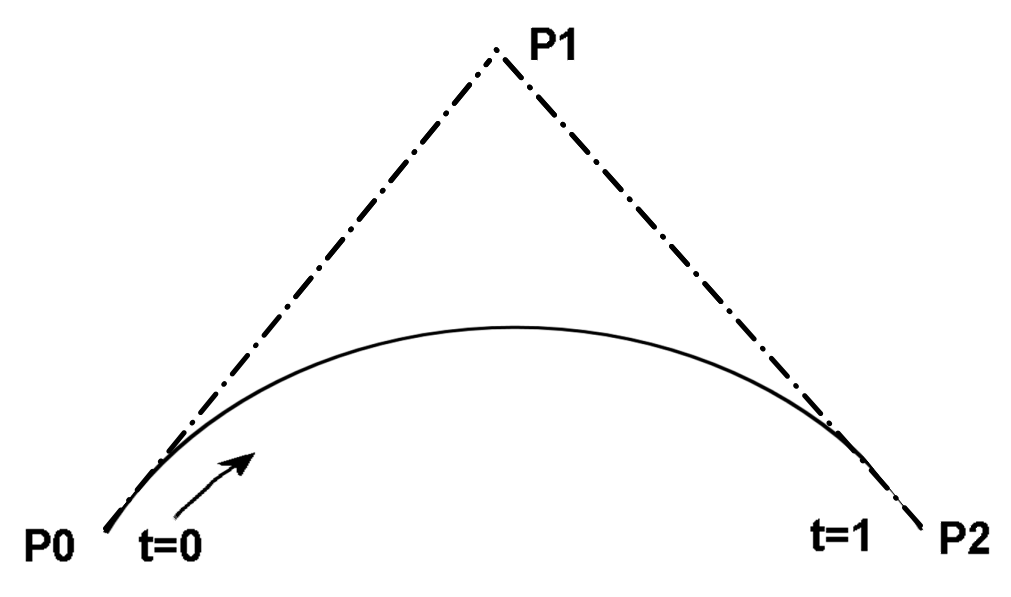
\includegraphics[width = 0.4\textwidth]{\fig/bez2.png}
\begin{displaymath}
\mathbf{x} = (1-t)^2\mathbf{p}_0 + 2t(1-t)\mathbf{p}_1 + t^2 \mathbf{p}_2
\end{displaymath}
%
\begin{myblock}{}{bg=smtbx,fg=black}{bg=smtbx, fg=red}
\begin{itemize}
\item Tangente in $t=0$: $2(\mathbf{p}_1-\mathbf{p}_0)$
\item Tangente in $t=1$: $2(\mathbf{p}_2-\mathbf{p}_1)$
\end{itemize}
\end{myblock}
\end{frame}
%
\begin{frame}
\frametitle{Curve di Bezier di ordine 3}
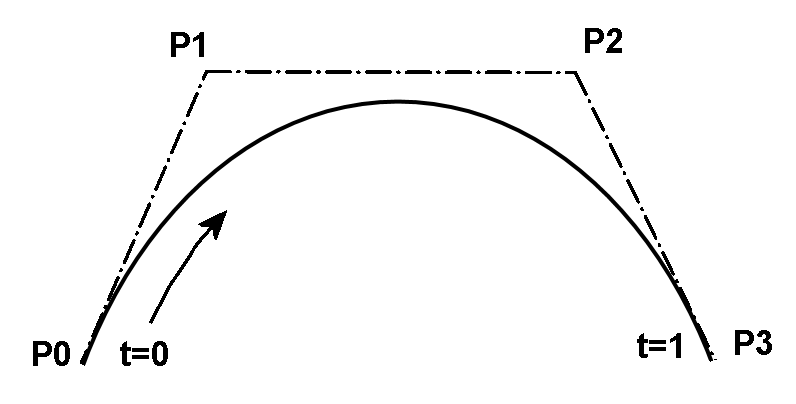
\includegraphics[width = 0.4\textwidth]{\fig/bez3.png}
\begin{displaymath}
\mathbf{x} = (1-t)^3\mathbf{p}_0 + 3 t(1-t)^2\mathbf{p}_1 + 3 t^2(1-t) \mathbf{p}_2+ t^3 \mathbf{p}_3
\end{displaymath}
\begin{myblock}{}{bg=smtbx,fg=black}{bg=smtbx, fg=red}
\begin{itemize}
\item Tangente in $t=0$: $3(\mathbf{p}_1-\mathbf{p}_0)$
\item Tangente in $t=1$: $3(\mathbf{p}_3-\mathbf{p}_2)$
\end{itemize}
\end{myblock}
\end{frame}
%
\begin{frame}
\frametitle{Esercizio 1}
\begin{itemize}
\item Rappresentare la curva di Bezier i cui punti di controllo siano:
\begin{align}
P_0 &= (0,0,0)\\
P_1 &= (1,0,3)\\
P_2 &= (2,0,1)
\end{align}
\item Indicare i punti di controllo.
\item Rappresentare le curva sia con il nodo `curve' che con il nodo  `Bezier Curve' e mostrare che i due risultati corrispondono.
\end{itemize}
\end{frame}
%
\begin{frame}
\frametitle{Esercizio 2 }
\begin{itemize}
\item Rappresentare la curva di Bezier i cui punti di controllo siano:
\begin{align}
P_0 &= (0,0,0) \\
P_1 &= (1,0,3)\\
P_2 &= (2,0,1)\\
P_3 &= (4,3,-1)
\end{align}
\item Rappresentare i punti di controllo e la curva.
\end{itemize}
\end{frame}
\begin{frame}[fragile]
\frametitle{Esercizi 1 e 2 - Risultati}
%\begin{myblock}{}{bg=smtbx,fg=black}{bg=smtbx, fg=red}
\begin{columns}
\begin{column}{0.5\textwidth}
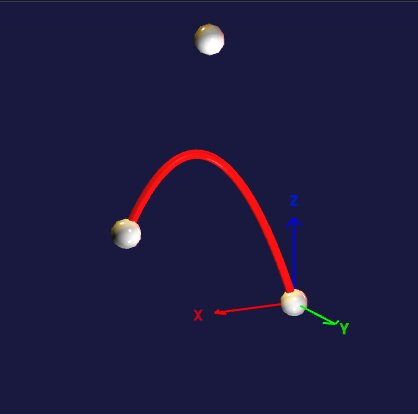
\includegraphics[width=\textwidth]{\fig/l6_bez2-1.jpeg}
\end{column}
\begin{column}{0.5\textwidth}
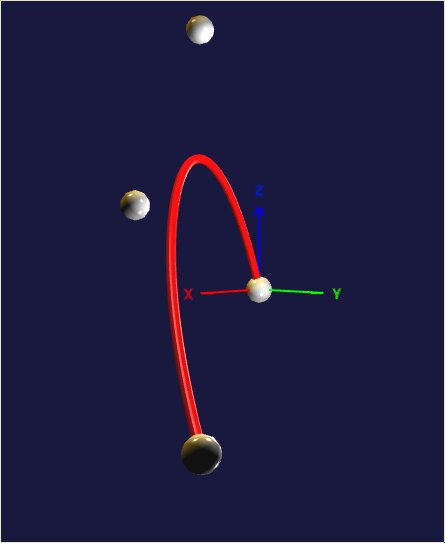
\includegraphics[width=\textwidth]{\fig/l6_bez3-1.jpeg}
\end{column}
\end{columns}
\end{frame}

%\section{Esercizi}
\begin{frame}
\frametitle{Esercizio 3}
\begin{itemize}
\item Rappresentare la curva di Bezier determinata dai punti
\begin{align}
P_0 &= (0,0,0 )\nonumber\\
P_1 &= (2,2,0 )\nonumber\\
P_2 &= (2,-2,0)\nonumber\\
P_3 &= (4,0,0 )\nonumber
\end{align}
\item Rappresentare una curva di Bezier di ordine a scelta il cui
punto di controllo iniziale ($Q_0$) corrisponda a $P_3$ ed il cui punto finale sia
(3,4,3).  Al variare dei punti di controllo che considerazioni si possono fare
sulle curve?
\end{itemize}
\end{frame}
\begin{frame}
\frametitle{Esercizio 3 - i}
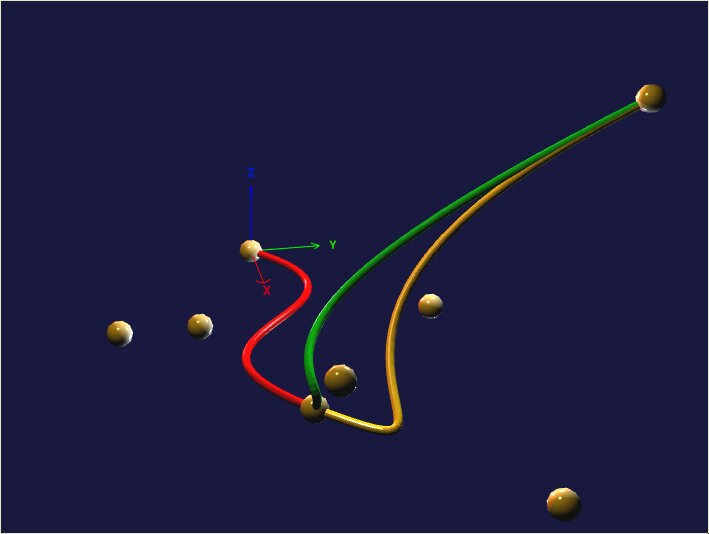
\includegraphics[width=\textwidth]{\fig/l6_es3.jpeg}
\end{frame}
\begin{frame}
\frametitle{Esercizio 4}
\begin{itemize}
\item Rappresentare la curva di Bezier data dai punti:
\begin{align}
P_0 &= (0,0,0)\nonumber\\
P_1 &= (1,0,0)\nonumber\\
P_2 &= (1,1,0)\nonumber\\
P_3 &= (1,1,1)\nonumber
\end{align}
\item Calcolare e rappresentare la curva riflessa rispetto al piano y-z.
\item Determinare se le due curve si raccordano con continuit\`a.
\end{itemize}
\begin{myblock}{\textbf{Nota}}{bg=smtbx,fg=black}{bg=smtbx, fg=red}
Con le curve di Bezier posso applicare la trasformazione richiesta ai punti di controllo, quindi scrivere la curva riflessa usando i punti riflessi
\end{myblock}
\end{frame}
%
\begin{frame}
\frametitle{Esercizio 4 - i}
\begin{columns}
\begin{column}{0.49\textwidth}
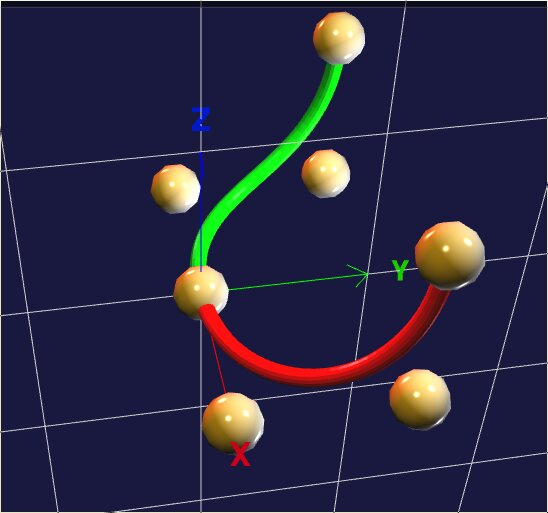
\includegraphics[width = \textwidth]{\fig/l6_es4.jpeg}
\end{column}
\begin{column}{0.49\textwidth}
%\includegraphics[width = \textwidth]{\fig/lab7_es2.png}
\end{column}
\end{columns}
\end{frame}
%
\begin{frame}
\frametitle{Esercizio 5}
\begin{itemize}
\item Rappresentare la curva  di Bezier $B1$ definita dai punti di controllo:
\begin{align}
P_0 &= (0,0,0 )\nonumber\\
P_1 &= (2,2,0 )\nonumber\\
P_2 &= (2,-2,0)\nonumber\\
P_3 &= (4,0,0 )\nonumber
\end{align}
\item Calcolare l'espressione della superficie che si ottiene traslando la curva $B1$  della curva $B2$ seguente:
\begin{align}
Q_0 &= (0,0,0)\nonumber\\
Q_1 &= (1,0,1)\nonumber\\
Q_2 &= (-2,-1,0)\nonumber\\
Q_3 &= (-1,4,3)\nonumber
\end{align}
\item Rappresentare la superficie e le curva $B2$.
\end{itemize}
\end{frame}
\begin{frame}
\frametitle{Esercizio 6}
\begin{itemize}
\item Fissati i punti:
\begin{align}
P_0 &= (0,0,0)\nonumber\\
P_1 &= (2,0,2)\nonumber\\
P_2 &= (1,-1,3)\nonumber\\
P_3 &= (0,1,3)\nonumber
\end{align}
\item Rappresentare la curva di Bezier, e la superficie che si ottiene componendo la curva con una rotazione di $2\pi$ attorno all'asse z.
\end{itemize}
\end{frame}
\begin{frame}
\frametitle{Esercizi 5-6}
\begin{columns}
\begin{column}{0.5\textwidth}
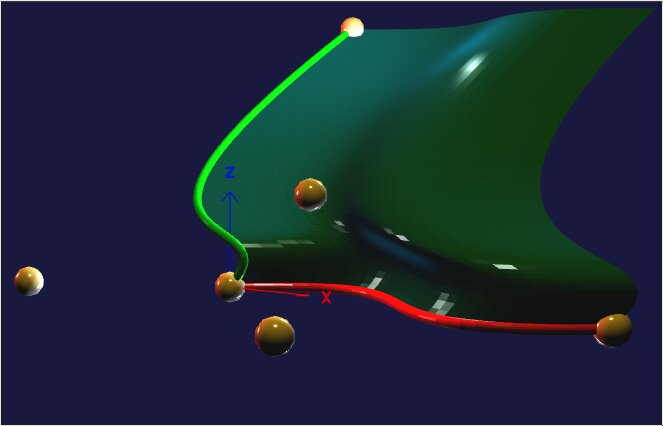
\includegraphics[width=\textwidth]{\fig/l6_es5.jpeg}
\end{column}
\begin{column}{0.5\textwidth}
$\mathbf{\longleftarrow}$\textbf{Es. 5}
\end{column}
\end{columns}
\begin{columns}
\begin{column}{0.5\textwidth}
\textbf{Es. 6}$~\mathbf{\longrightarrow}$
\end{column}
\begin{column}{0.5\textwidth}
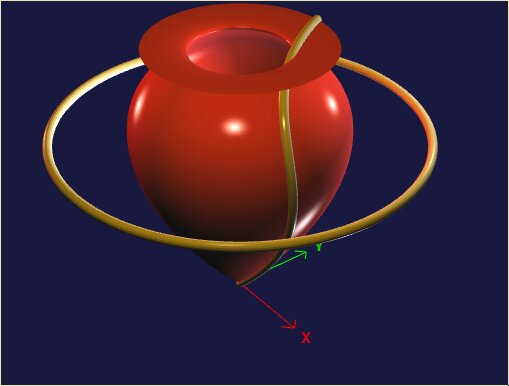
\includegraphics[width=\textwidth]{\fig/l6_es6.jpeg}
\end{column}
\end{columns}
%\begin{itemize}
%\item Data la curva di Bezier definita dai punti:
%\begin{align}
%P_0 &= [0,0,0]^T\\
%P_1 &= [0,1,1]^T\\
%P_2 &= [-1,2,3]^T\\
%P_3 &= [0,0,3]^T
%\end{align}
%\item Disegnare i due piani definiti dai due punti $P_1$ e $P_2$ e dalle tangenti della curva in $P_0$ e $P_3$, rispettivamente.
%\end{itemize}
\end{frame}
%% %%%% Raccordo tra le curve
\begin{frame}
\frametitle{Raccordo tra curve di Bezier - i}
Data una curva definita dai punti $P_0$, $P_1$, $P_2$, $P_3$ e dal parametro $t$ e la curva definita dai punti $Q_0$, $Q_1$, $Q_2$, $Q_3$ e dal parametro $s$, \`e possibile raccordarle in 4 modi.
\begin{columns}
\begin{column} {0.49\textwidth}

\begin{itemize}
\item $\mathbf{p}_0= \mathbf{q}_3$: $t=0$, $s = 1$ 
e $3(\mathbf{p}_1-\mathbf{p}_0) = 3(\mathbf{q}_3-\mathbf{q}_2)$ (\textbf{Caso A});
\item  $\mathbf{p}_3 = \mathbf{q}_0$: $t=1$, $s = 0$ e $3(\mathbf{p}_3-\mathbf{p}_2) = 3(\mathbf{q}_1-\mathbf{q}_0)$ (\textbf{Caso B});
\end{itemize}
\end{column}
\begin{column} {0.49\textwidth}
\begin{itemize}
\item $\mathbf{p}_0= \mathbf{q}_0$: $t=0$, $s =0$ e $3(\mathbf{p}_1-\mathbf{p}_0) = -3(\mathbf{q}_1-\mathbf{q}_0)$ (\textbf{Caso C});
\item  $\mathbf{p}_3 = \mathbf{q}_3$: $t=1$, $s = 1$ e $3(\mathbf{p}_3-\mathbf{p}_2) = -3(\mathbf{q}_3-\mathbf{q}_2)$ (\textbf{Caso D});
\end{itemize}
\end{column}
\end{columns}
\vspace{1cm}
\textbf{Nota: nei casi C e D la connessione \`e liscia ma non c'\`e continuit\`a della tangente!! (cambio di segno)}
\end{frame}
%
\begin{frame}
\frametitle{Raccordo tra curve di Bezier - ii}
\begin{columns}
\begin{column}{0.6\textwidth}
\begin{tikzpicture}
\node[anchor=center, inner sep = 0](image)at (0,0) {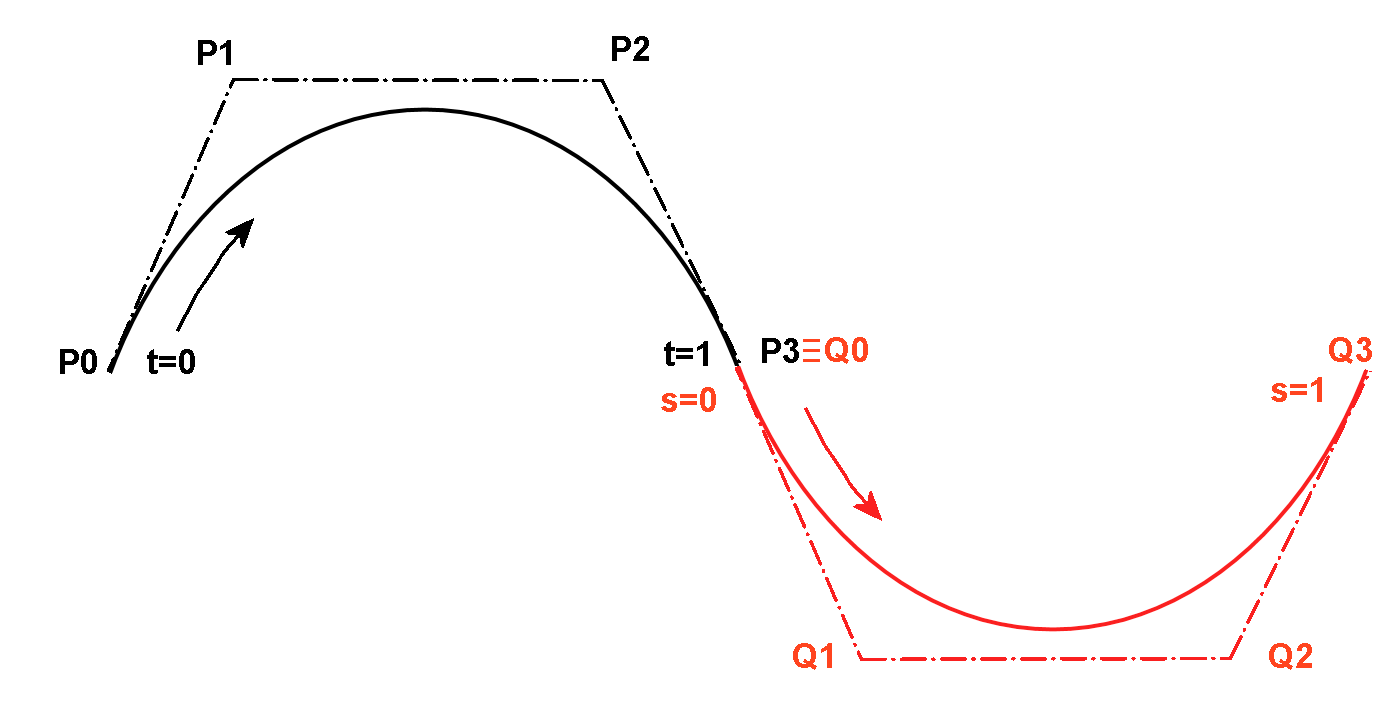
\includegraphics[width=\textwidth]{\fig/bezcon_A.png}};
\node[align=center,blue,font={\bfseries}] at (image.north west) {Caso A};
\end{tikzpicture}
\end{column}
\begin{column}{0.3\textwidth}
\begin{tikzpicture}
\node[anchor=center, inner sep = 0](image)at (0,0) {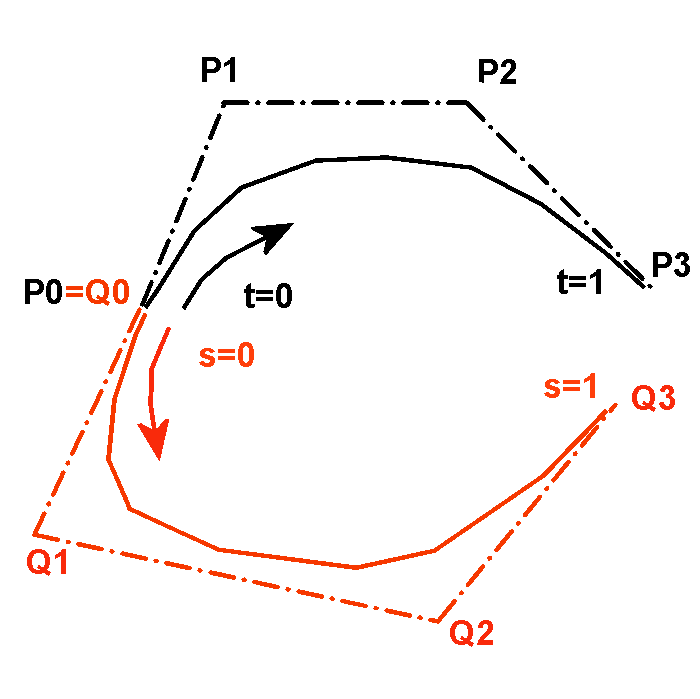
\includegraphics[width=\textwidth]{\fig/bezcon_C.png}};
\node[align=center,blue,font={\bfseries}] at (image.north west) {Caso C};
\end{tikzpicture}
\end{column}
\end{columns}
\begin{columns}
\begin{column}{0.3\textwidth}
\begin{tikzpicture}
\node[anchor=center, inner sep = 0](image)at (0,0) {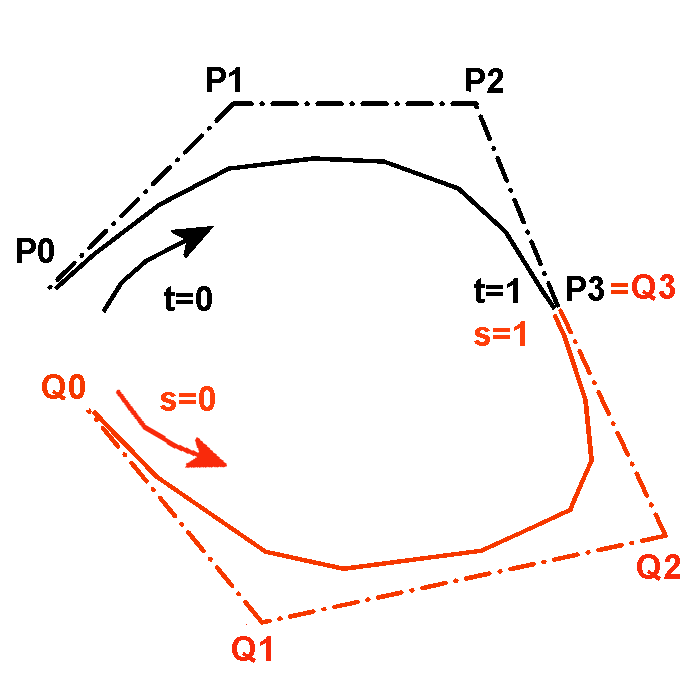
\includegraphics[width=\textwidth]{\fig/bezcon_D.png}};
\node[align=center,blue,font={\bfseries}] at (image.north west) {Caso D};
\end{tikzpicture}
\end{column}
\begin{column}{0.6\textwidth}
\begin{tikzpicture}
\node[anchor=center, inner sep = 0](image)at (0,0) {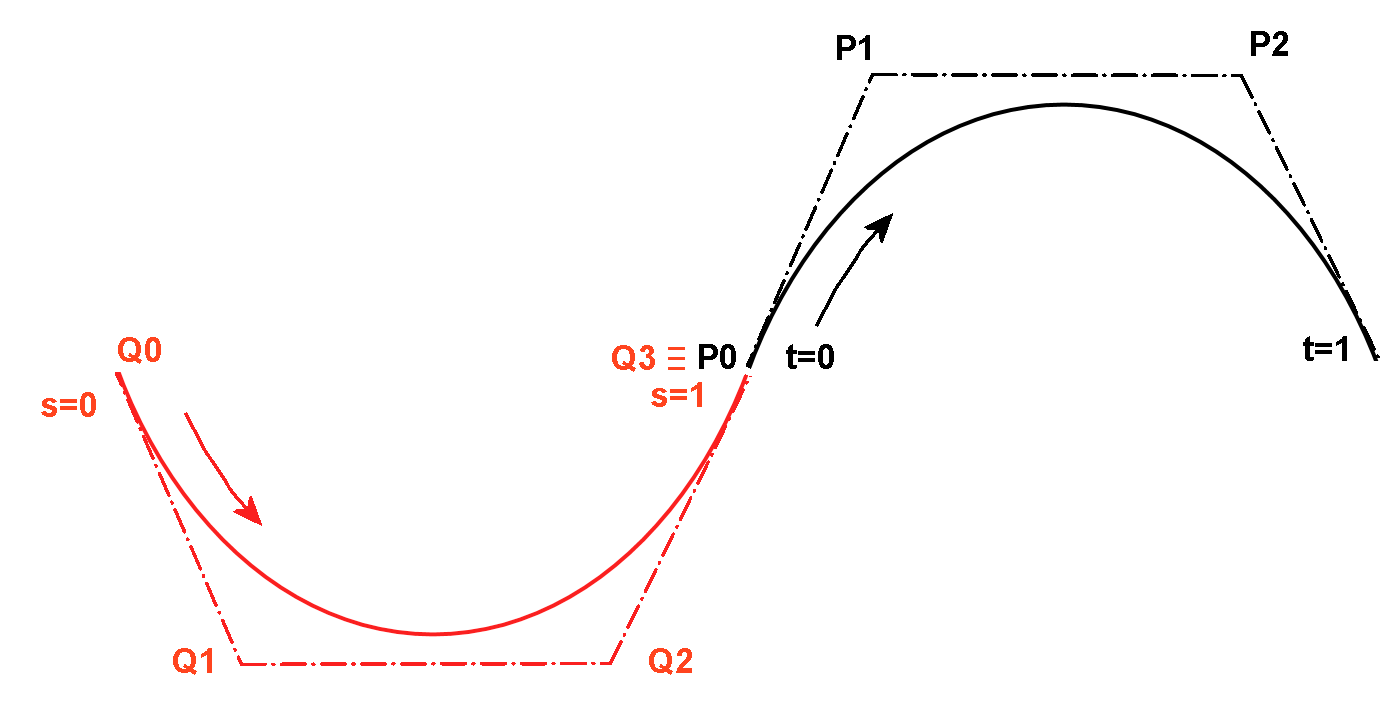
\includegraphics[width=\textwidth]{\fig/bezcon_B.png}};
\node[align=center,blue,font={\bfseries}] at (image.south east) {Caso B};
\end{tikzpicture}
\end{column}
\end{columns}
\end{frame}


\end{document}
